%%
%% This is file `sample-acmlarge.tex',
%% generated with the docstrip utility.
%%
%% The original source files were:
%%
%% samples.dtx  (with options: `acmlarge')
%% 
%% IMPORTANT NOTICE:
%% 
%% For the copyright see the source file.
%% 
%% Any modified versions of this file must be renamed
%% with new filenames distinct from sample-acmlarge.tex.
%% 
%% For distribution of the original source see the terms
%% for copying and modification in the file samples.dtx.
%% 
%% This generated file may be distributed as long as the
%% original source files, as listed above, are part of the
%% same distribution. (The sources need not necessarily be
%% in the same archive or directory.)
%%
%%
%% Commands for TeXCount
%TC:macro \cite [option:text,text]
%TC:macro \citep [option:text,text]
%TC:macro \citet [option:text,text]
%TC:envir table 0 1
%TC:envir table* 0 1
%TC:envir tabular [ignore] word
%TC:envir displaymath 0 word
%TC:envir math 0 word
%TC:envir comment 0 0
%%
%%
%% The first command in your LaTeX source must be the \documentclass command.
\documentclass[acmlarge]{acmart}
\usepackage{listings}
\lstset{language=Go,
  basicstyle=\ttfamily\scriptsize,
  keywordstyle=\color{blue}\ttfamily,
  stringstyle=\color{red}\ttfamily,
  commentstyle=\color{green}\ttfamily}
%%ss[STYLE]{acmart}
%% \BibTeX command to typeset BibTeX logo in the docs
\AtBeginDocument{%
  \providecommand\BibTeX{{%
    \normalfont B\kern-0.5em{\scshape i\kern-0.25em b}\kern-0.8em\TeX}}}

%% Rights management information.  This information is sent to you
%% when you complete the rights form.  These commands have SAMPLE
%% values in them; it is your responsibility as an author to replace
%% the commands and values with those provided to you when you
%% complete the rights form.
\setcopyright{acmcopyright}
\copyrightyear{2022}
\acmYear{2022}
\acmDOI{}


%%
%% These commands are for a JOURNAL article.
\acmJournal{POMACS}
\acmVolume{37}
\acmNumber{4}
\acmArticle{8}
\acmMonth{8}

%%
%% Submission ID.
%% Use this when submitting an article to a sponsored event. You'll
%% receive a unique submission ID from the organizers
%% of the event, and this ID should be used as the parameter to this command.
%%\acmSubmissionID{123-A56-BU3}

%%
%% The majority of ACM publications use numbered citations and
%% references.  The command \citestyle{authoryear} switches to the
%% "author year" style.
%%
%% If you are preparing content for an event
%% sponsored by ACM SIGGRAPH, you must use the "author year" style of
%% citations and references.
%% Uncommenting
%% the next command will enable that style.
%%\citestyle{acmauthoryear}

%%
%% end of the preamble, start of the body of the document source.
\begin{document}

%%
%% The "title" command has an optional parameter,
%% allowing the author to define a "short title" to be used in page headers.
\title{Paper Reading of \textit{TensorFlow: A System for Large-Scale Machine Learning}}

%%
%% The "author" command and its associated commands are used to define
%% the authors and their affiliations.
%% Of note is the shared affiliation of the first two authors, and the
%% "authornote" and "authornotemark" commands
%% used to denote shared contribution to the research.
\author{Yiwei Yang}
\email{yangyw@shanghaitech.edu.cn}
\orcid{0000-0001-8011-5868}
\affiliation{
  \institution{ShanghaiTech University}
  \streetaddress{1 R.D. Zhongke}
  \city{Shanghai}
  \state{Shanghai}
  \country{China}
  \postcode{21210}
}

%%
%% By default, the full list of authors will be used in the page
%% headers. Often, this list is too long, and will overlap
%% other information printed in the page headers. This command allows
%% the author to define a more concise list
%% of authors' names for this purpose.
\renewcommand{\shortauthors}{Yiwei Yang}

%%
%% The abstract is a short summary of the work to be presented in the
%% article.
\begin{abstract}
Because its predecessor, DistBelief, was too rigid for various types of ML work Large-scale training, small-scale service, and research are the three categories of ML work. DistBelief was fast for large-scale training, but if you want to scale down your training to run in a tiny environment with a small dataset or conduct research with new layers, you'll need to update the C++ code.

So Tensorflow \cite{abadi2016tensorflow} has Parameter servers are distributed key-value stores that keep track of the status of model parameters. Moreover, Workers read data from disk, execute mathematical computations, and update model parameters using parameter servers to drive the training process. These workers are usually powered by a high-performance CPU or GPU.
\begin{figure}[htbp]
  \centering
  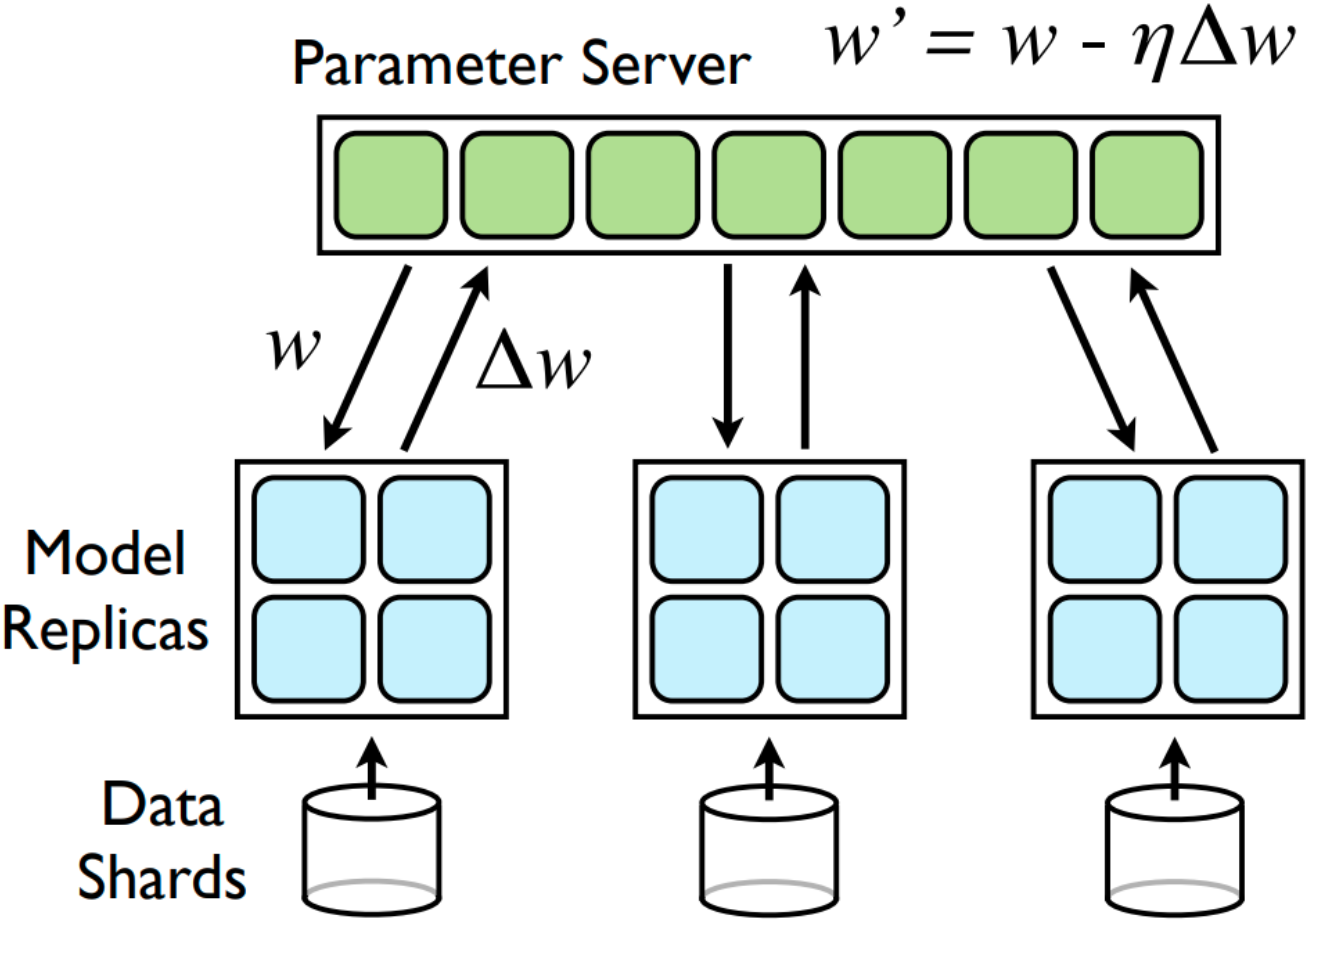
\includegraphics[width=10cm]{./workers.png}
  \caption{Workers fetch parameters w and push gradients $\delta$w to parameter servers.}
\end{figure}
\end{abstract}

%%
%% The code below is generated by the tool at http://dl.acm.org/ccs.cfm.
%% Please copy and paste the code instead of the example below.
%%
\begin{CCSXML}
  <ccs2012>
  <concept>
  <concept_id>10010520.10010553.10010562</concept_id>
  <concept_desc>Distributed System~Peer to Peer System</concept_desc>
  <concept_significance>500</concept_significance>
  </concept>
  </ccs2012>
\end{CCSXML}

\ccsdesc[500]{Distributed System~Distributed Hash Table}

%%
%% Keywords. The author(s) should pick words that accurately describe
%% the work being presented. Separate the keywords with commas.
\keywords{Tensor computation, parameter propogation}

%%
%% This command processes the author and affiliation and title
%% information and builds the first part of the formatted document.
\maketitle
\section{Strong point of the document}

\subsection{Effectiveness of combining parameters communication and labour server utilization}
There is no differentiation between a parameter server process and a worker process in TensorFlow. The implementation is the same for all processes. A stateful or stateless process can exist. Stateful ones, which act like parameter servers, feature a mutable buffer to hold model parameters. Stateless individuals can concentrate on crunching numbers and communicating with stateful individuals to get and set those parameters, effectively acting as laborers.
\begin{figure}[htbp]
  \centering
  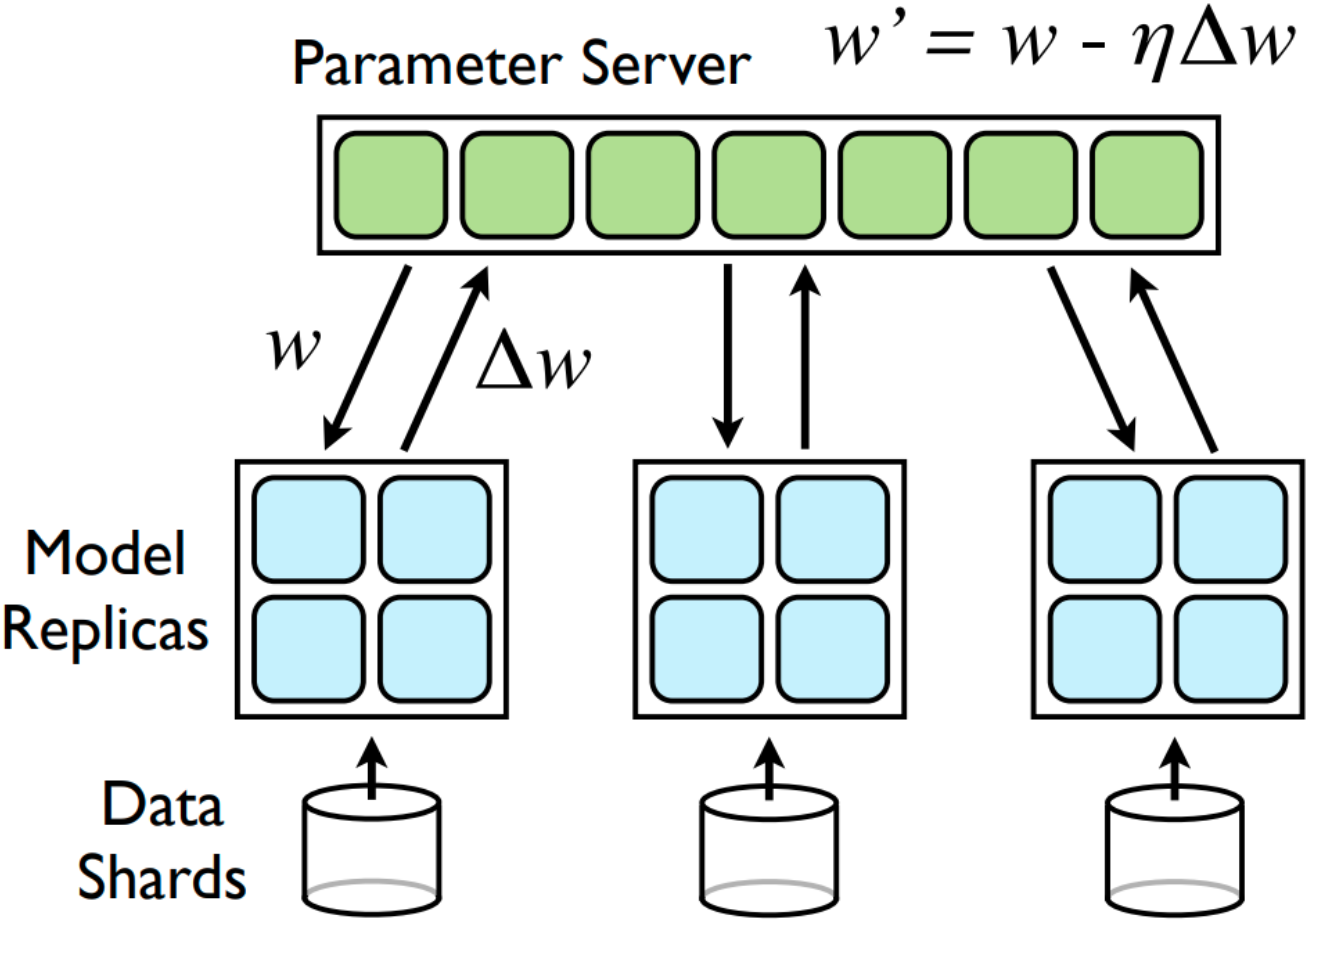
\includegraphics[width=5cm]{./workers.png}
\end{figure}
A tensor is a multi-dimensional array. Tensors flow along edges in a dataflow graph where vertices are operations.
\begin{figure}[htbp]
  \centering
  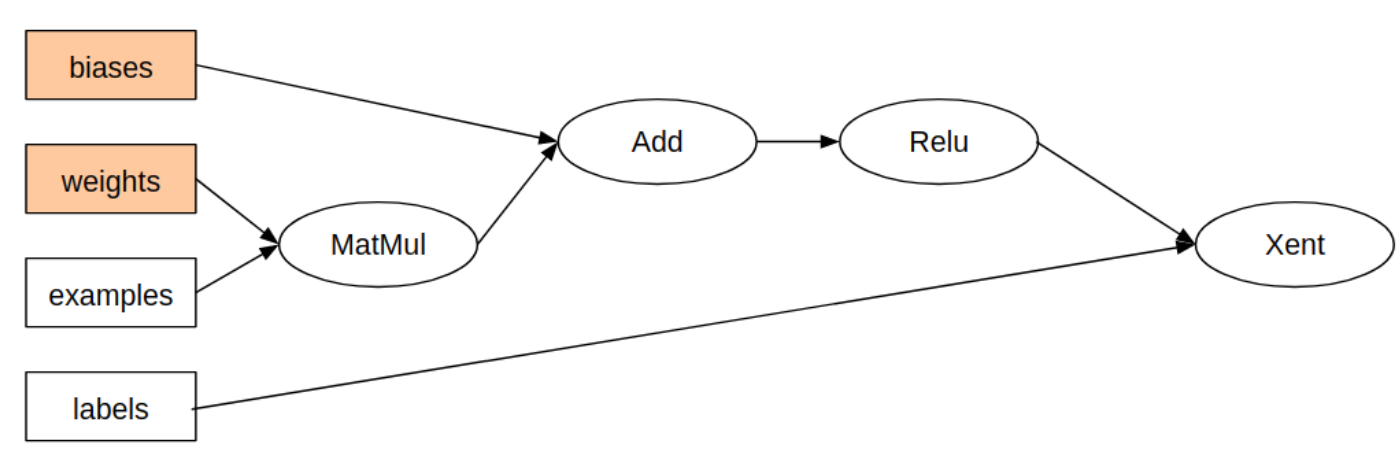
\includegraphics[width=5cm]{./tensor.png}
\end{figure}

\subsection{Multiple Language Backends for Graph Computation}
For efficiency, the TensorFlow runtime is written in C++. Python, Go, Java, C++, and other languages can be used for user-level code. Programmers create a graph, designate the node(s) for which they want a value (fetch), and supply input data. The following is what the TensorFlow runtime does with the graph.
\begin{enumerate}
\item Partial execution graph pruning: TensorFlow examines the graph and only performs the calculations required to compute the fetch.
\item A TensorFlow workflow can have several subgraphs running at the same time. Some subgraphs are run in parallel, such as concurrent preprocessing, which modifies incoming data independently. Concurrent subgraphs such as concurrent training, where parameters are changed based on various input batches, interact through shared variables and queues.
\item TensorFlow's runtime distributes actions across different devices. Computationally intensive operations are performed on GPUs by default, while stateful bookkeeping functions are placed on CPUs. Users have the ability to customize their own placement. The problem of determining the best device location automatically is still under investigation. On each edge that traverses devices, the TensorFlow runtime inserts a communication channel.
\end{enumerate}
\begin{figure}[htbp]
  \centering
  \caption{A dataflow graph is divided into sections and spread across multiple devices. A GPU is used for processes that need a lot of math. On a CPU, stateful bookkeeping operations are performed. TensorFlow runtime inserts a send-receive channel whenever an edge passes between devices.}
  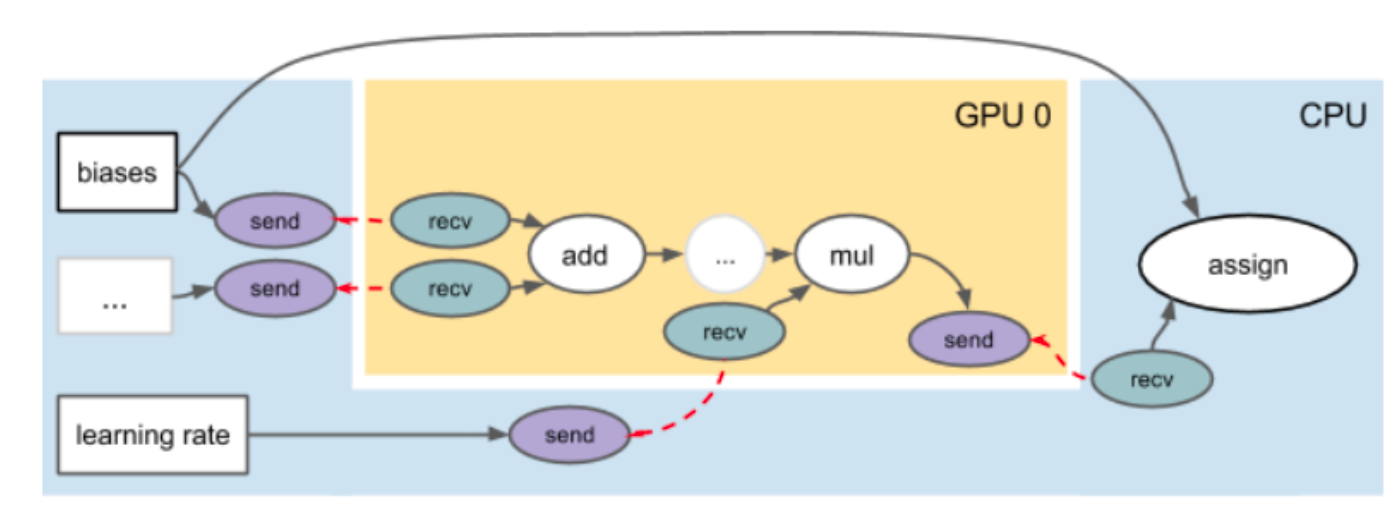
\includegraphics[width=5cm]{./gpu.png}
\end{figure}
\subsection{Dynamic Control Flow in TensorFlow}
Conditional and iterative control flows are used in several sophisticated machine learning methods (e.g., recurrent neural networks and reinforcement learning). The goal of dynamic control flow in a machine learning framework is to provide conditionals and loops through a TensorFlow interface (in-graph control flow). Programmers must rely on user-level language conditional and loop constructions in the absence of in-graph control flow (out-of-graph control flow). TensorFlow defines control-flow primitives (e.g. switch, merge, nextIteration) to express conditional and loop constructs. As a result, conditionals and loops can be represented graphically. In-graph control flow allows TensorFlow to process and optimize a single unified graph, thus allowing more parallelism and distribution.
\begin{figure}[htbp]
  \centering
  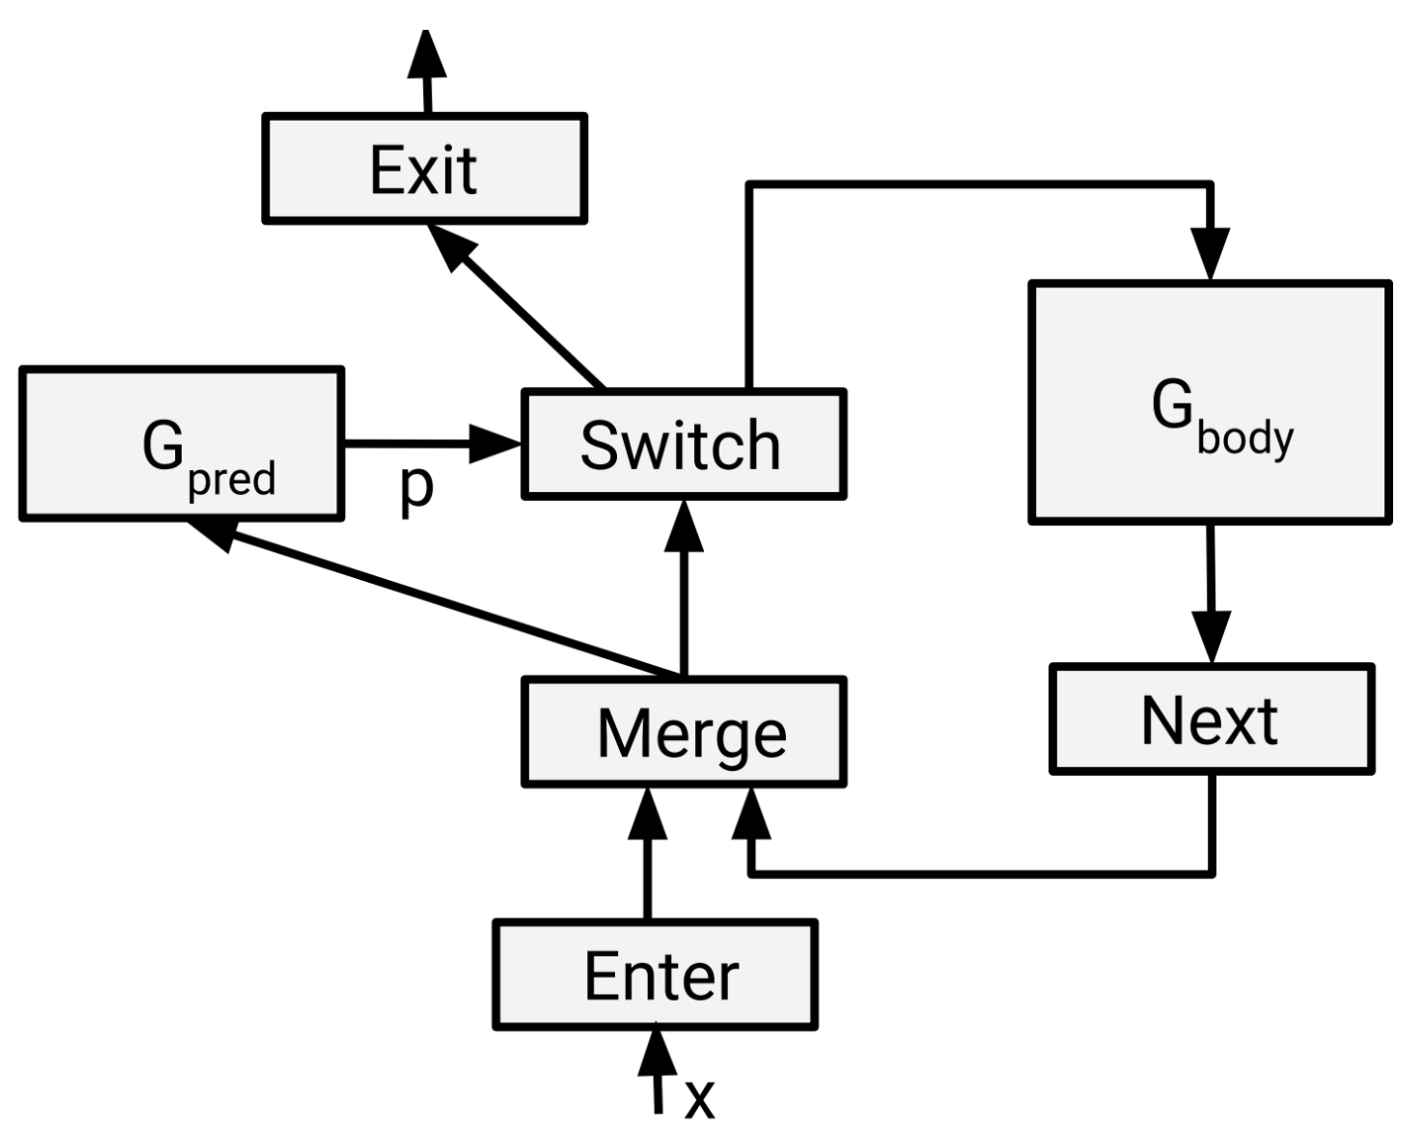
\includegraphics[width=5cm]{./primitive.png}
\end{figure}
\section{Weak point of the document}
\subsection{The ecosystem of tensorflow is not as strong as pytorch}
PyTorch is much easier to use (you can tell how unfriendly a framework itself is when it can derive many upper-level frameworks, speaking of TF), and the ecology is up, with most papers open-sourced with PyTorch. For PyTorch, If it is a computational graph for backpropagation, the gradient is calculated from the last node after you call backward, and then as soon as the inputs of an operator are ready, the operator is scheduled to execute\dots
\subsection{The original implementation's synchronous replica coordination is not scalable}
Some people have recently re-examined the idea that synchronous training isn't scaleable. Because GPUs enable training with hundreds rather than thousands of computers, synchronous training on the same platform may be faster (in terms of time to quality). Use queues to implement the synchronous version. A blocking queue ensures that all workers read the same parameter values, while a per-variable queue collects gradient updates from all workers and applies them atomically.
\begin{figure}[htbp]
  \centering
  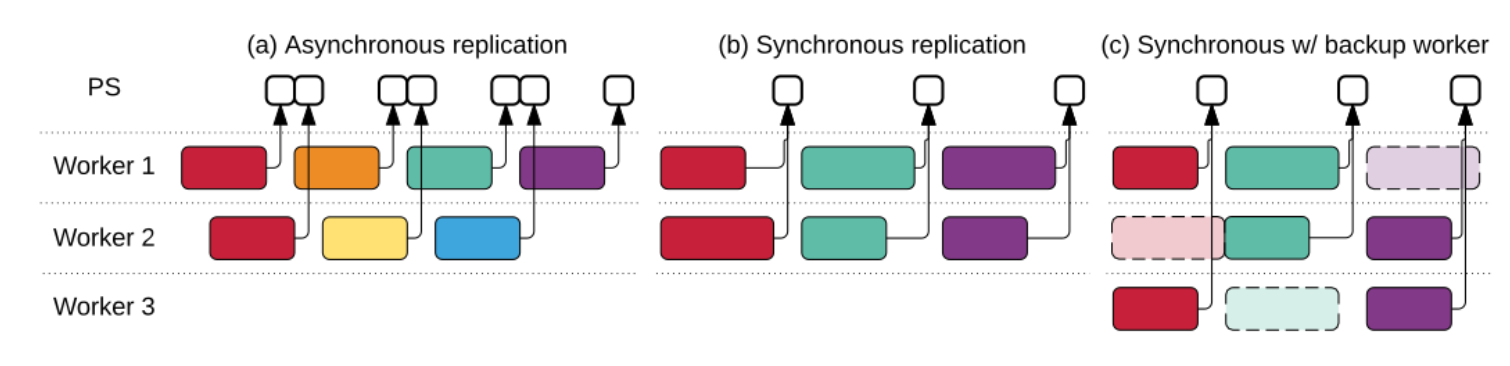
\includegraphics[width=5cm]{./replica.png}
\end{figure}
\begin{figure}[htbp]
  \centering
  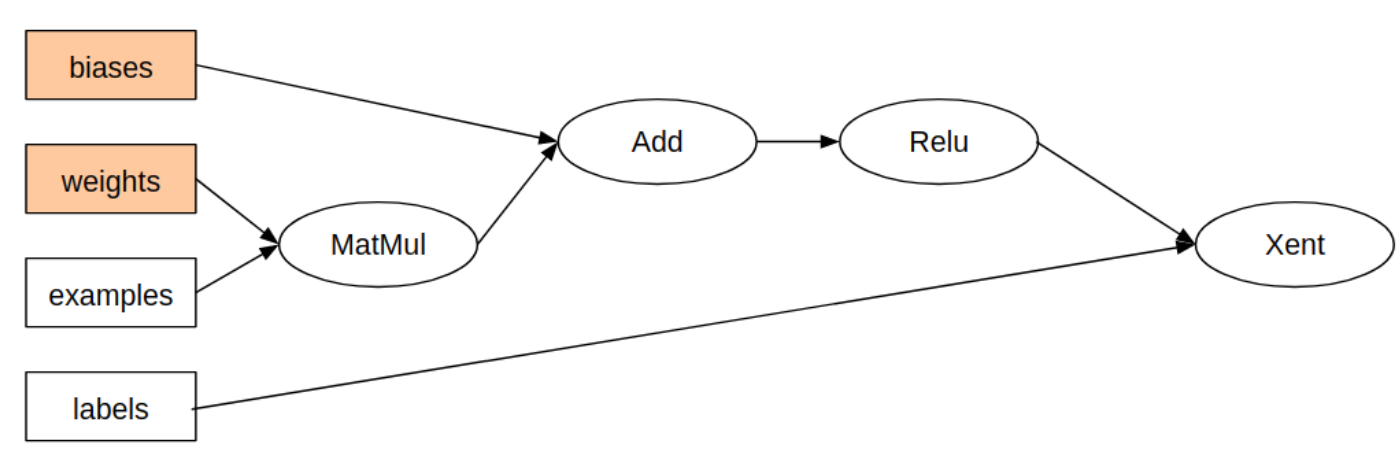
\includegraphics[width=5cm]{./tensor.png}
  \caption{Different execution flow.  Synchronous and Asynchronous}
\end{figure}
\section{Possible refinement}
\subsection{The graph optimization can be based on a intermediate representation}
After the appearance of TVM\cite{chen2018tvm}, we notice that with the growing of backend devices, we have to design a intermediate representation to represent the graph. The tensorflow has already a middle ware called MLIR(Multi Level Intermediate Representation) to generate code to
\subsection{JIT compilations }
Every time we may have consume a lot of time recompiling and deploying data. The Just in Time compilation can both utilize the runtime graph information for better Cuda kernel generation and faster compilation overall.
\subsection{The communication between servers are based is non confidential}
We can apply the federated learning method to better improve the data and parameter updates \cite{federated}. For example, we can apply encryption and decryption to the passing variables of asynchronous SGD which does not hurt the precision of data and parameter updates.
\bibliographystyle{ACM-Reference-Format}
\bibliography{tensorFlow_a_system_for_large_scale_machine_learning}
\end{document}
\endinput
%%
%% End of file `sample-acmlarge.tex'.
